\documentclass[11pt]{article}
\usepackage{../../latex/stat4ml_style}

\title{Chapter 6: Maximum Likelihood Estimation \\ \large Part I --- Statistics Foundation for ML}
\author{Omid Safarzadeh}
\date{}

\begin{document}
\maketitle

\begin{abstract}
\noindent
Maximum likelihood is the estimation principle underneath most of modern
machine learning. Faced with data and a model that has an unknown
parameter, it asks a single question --- which value of the parameter would
have made the data we actually observed most probable? --- and takes the
answer as the estimate. This chapter develops that idea in full: we define
the likelihood, compute the estimator for the models you meet most often,
and then ask how good it is, arriving at the score, the Fisher information,
the Cram\'er--Rao lower bound, and the fact that the estimator is
asymptotically normal. A final section looks at what happens when the usual
assumptions fail, and shows that maximising the likelihood is the same as
minimising a Kullback--Leibler divergence --- the sentence that ties this
chapter to every cross-entropy loss you will later minimise.
\end{abstract}

\tableofcontents

% ======================================================================
\section{The likelihood and the maximum-likelihood estimator}
% ======================================================================

Suppose we observe data $x_1,\dots,x_n$, modelled as independent draws from
a density (or mass function) $f(x\,;\theta)$ with an unknown parameter
$\theta$. The density answers a forward question: with $\theta$ fixed, how
probable is each possible value of $x$? Estimation runs that question
backwards. The data are now in hand and fixed; it is $\theta$ we do not
know. Reading the same formula with the data fixed and $\theta$ free gives
the \keyterm{likelihood}: how probable were the numbers we actually saw, as
a function of the parameter that might have produced them?

\begin{definition}[Likelihood and log-likelihood]
For independent observations the \emph{likelihood} is
\[
  L(\theta) = \prod_{i=1}^{n} f(x_i\,;\theta),
  \qquad
  \ell(\theta) = \log L(\theta) = \sum_{i=1}^{n} \log f(x_i\,;\theta).
\]
The \emph{maximum-likelihood estimator} (MLE) is the value that makes the
observed data most probable,
\[
  \hat\theta = \arg\max_{\theta} L(\theta) = \arg\max_{\theta} \ell(\theta).
\]
\end{definition}

We almost always maximise the log-likelihood $\ell$ rather than $L$ itself,
and for three reasons. The logarithm is strictly increasing, so it does not
move the location of the maximum; it turns the product into a sum, which we
can differentiate term by term; and it replaces the multiplication of
thousands of small probabilities, which underflows to zero in floating
point, by the addition of their logarithms, which does not. In the smooth
case we then find the maximum the usual way: solve the \keyterm{likelihood
equation} $\ell'(\theta)=0$ and confirm the solution is a maximum rather
than a minimum or a saddle. The three examples below are the ones worth
knowing by heart.

\begin{example}[Bernoulli]
For $x_i\in\{0,1\}$ independent and $\mathrm{Bernoulli}(p)$,
\[
  \ell(p) = \Big(\textstyle\sum_i x_i\Big)\log p
          + \Big(n-\textstyle\sum_i x_i\Big)\log(1-p),
  \qquad
  \ell'(p) = \frac{\sum_i x_i}{p} - \frac{n-\sum_i x_i}{1-p}.
\]
Setting $\ell'(p)=0$ gives $\hat p = \bar x$: the maximum-likelihood
estimate of a probability is just the observed proportion.
\end{example}

\begin{example}[Normal]
For $x_i$ independent and $N(\mu,\sigma^2)$,
\[
  \ell(\mu,\sigma^2) = -\frac{n}{2}\log(2\pi\sigma^2)
     - \frac{1}{2\sigma^2}\sum_{i=1}^n (x_i-\mu)^2 ,
\]
and solving the two likelihood equations (one for $\mu$, one for
$\sigma^2$) gives
\[
  \hat\mu = \bar x,
  \qquad
  \hat\sigma^2 = \frac{1}{n}\sum_{i=1}^n (x_i-\bar x)^2 .
\]
\end{example}

\begin{example}[Poisson]
For $x_i$ independent and $\mathrm{Poisson}(\lambda)$ we have
$\ell(\lambda)=\big(\sum_i x_i\big)\log\lambda - n\lambda - \sum_i\log(x_i!)$,
so once again $\hat\lambda = \bar x$.
\end{example}

Every one of these estimators is a one-liner once you have the formula.
Here are four of them side by side, in plain Python --- the kind of
side-by-side that makes maximum likelihood click:

\begin{lstlisting}[language=Python]
def mle_bernoulli(x):   return sum(x) / len(x)        # p_hat      = mean
def mle_poisson(x):     return sum(x) / len(x)        # lambda_hat = mean
def mle_exponential(x): return len(x) / sum(x)        # rate       = 1 / mean
def mle_normal(x):
    mu  = sum(x) / len(x)
    var = sum((xi - mu)**2 for xi in x) / len(x)      # divide by n: the MLE
    return mu, var

print(mle_bernoulli([1, 1, 0, 1, 0]))         # -> 0.6
print(mle_poisson([2, 1, 3, 0, 2, 1, 4, 2]))  # -> 1.875
print(mle_exponential([0.4, 1.2, 0.9, 2.1]))  # -> 0.8695...
print(mle_normal([2, 4, 4, 4, 5, 5, 7, 9]))   # -> (5.0, 4.0)
\end{lstlisting}

\noindent The recipe never changes: write down $\ell(\theta)$, set
$\ell'(\theta)=0$, read off the estimator. The R versions sit beside these
in the chapter's \texttt{exercises/} folder.

\begin{editorialnote}
Notice that the normal variance estimate divides by $n$, not by $n-1$. The
maximum-likelihood estimator is therefore \emph{biased}:
$E[\hat\sigma^2] = \frac{n-1}{n}\sigma^2$, a little too small on average.
This is not a mistake to be corrected --- it is what maximum likelihood
does. The method optimises the fit to the sample actually observed and
makes no promise of unbiasedness; the next section makes the trade-off
precise. (The deliberately planted bug in this chapter's first exercise is
exactly this $n$-versus-$(n-1)$ slip.)
\end{editorialnote}

\subsection*{A cookbook of estimators}

The same recipe --- write down $\ell(\theta)$, solve $\ell'(\theta)=0$ ---
produces a one-line estimator for most of the distributions you will meet.
The common closed forms are collected below; a runnable version of every one,
in Python and R, sits beside this chapter in \texttt{mle\_cookbook.py} and
\texttt{mle\_cookbook.R}.

\begin{center}
{\small
\renewcommand{\arraystretch}{1.35}
\begin{tabular}{@{}ll@{}}
\hline
\textbf{Distribution} & \textbf{Maximum-likelihood estimate} \\
\hline
Bernoulli$(p)$ & $\hat p = \bar x$ \\
Binomial$(k,p)$, $k$ known & $\hat p = \bar x / k$ \\
Geometric$(p)$ & $\hat p = 1/\bar x$ \\
Poisson$(\lambda)$ & $\hat\lambda = \bar x$ \\
Exponential$(\lambda)$ & $\hat\lambda = 1/\bar x$ \\
Normal$(\mu,\sigma^2)$ & $\hat\mu=\bar x,\quad \hat\sigma^2=\tfrac1n\sum_i (x_i-\bar x)^2$ \\
Uniform$(0,\theta)$ & $\hat\theta=\max_i x_i$ \\
Laplace$(\mu,b)$ & $\hat\mu=\operatorname{median}(x),\quad \hat b=\tfrac1n\sum_i|x_i-\hat\mu|$ \\
Pareto$(x_m,\alpha)$, $x_m$ known & $\hat\alpha = n\big/\sum_i \log(x_i/x_m)$ \\
Gamma$(k,\theta)$, $k$ known & $\hat\theta=\bar x/k$ \\
\hline
\end{tabular}
}
\end{center}

\noindent When no closed form exists --- the Gamma with both parameters free,
the Weibull, the Beta --- the recipe is unchanged; you solve
$\ell'(\theta)=0$ numerically, with Newton's method on the score. The cookbook
includes one such example.

% ======================================================================
\section{Score, information, and the quality of the estimator}
% ======================================================================

Computing the estimator is only half the job. We also want to know how much
to trust it: how sharply the likelihood peaks around $\hat\theta$, and
whether any other estimator could do better. Both questions are answered by
two quantities built from the derivative of the log-likelihood --- the
score and the Fisher information.

\begin{definition}[Score and Fisher information]
The \keyterm{score} is the derivative of the log-likelihood,
$U(\theta)=\dfrac{\partial \ell}{\partial\theta}$. The \keyterm{Fisher
information} is its variance,
\[
  I_n(\theta) = \operatorname{Var}_\theta\!\big(U(\theta)\big)
              = E_\theta\!\big[U(\theta)^2\big].
\]
For $n$ independent observations $I_n(\theta)=n\,I_1(\theta)$, where $I_1$
is the information carried by a single observation.
\end{definition}

The score measures how strongly the data push the estimate up or down at a
given $\theta$; at the maximum the push vanishes, which is just the
likelihood equation $U(\hat\theta)=0$. Two facts make the score the right
object to study. The first is that, averaged over datasets drawn from the
model at the true $\theta$, it is zero.

\begin{theorem}[The score has mean zero]
Under the regularity conditions of Section 3, $E_\theta[U(\theta)] = 0$.
\end{theorem}
\begin{proof}
Work with a single observation; summing over $i$ gives the general case.
Because $f(\cdot\,;\theta)$ is a density it integrates to $1$ for every
$\theta$, so $\frac{\partial}{\partial\theta}\int f(x;\theta)\,dx = 0$.
Exchanging the derivative and the integral --- this is the regularity
assumption --- and using $\partial_\theta f = f\,\partial_\theta\log f$,
\[
  0 = \int \frac{\partial}{\partial\theta} f(x;\theta)\,dx
    = \int \big(\partial_\theta \log f(x;\theta)\big) f(x;\theta)\,dx
    = E_\theta\!\big[\partial_\theta \log f(X;\theta)\big] = E_\theta[U]. \qedhere
\]
\end{proof}

Differentiating that identity once more gives a second fact, which is the
reason the information can be computed two different ways --- as the
variance of the score, or as the curvature of the log-likelihood.

\begin{theorem}[Information identity]
Under regularity, $I_1(\theta) = -\,E_\theta\!\big[\partial_\theta^2 \log f(X;\theta)\big]$.
\end{theorem}
\begin{proof}
Differentiate $\int (\partial_\theta\log f)\,f\,dx=0$ with respect to
$\theta$:
\[
  0 = \int \big(\partial_\theta^2\log f\big) f\,dx
    + \int \big(\partial_\theta\log f\big)\big(\partial_\theta f\big)\,dx
    = E\!\big[\partial_\theta^2\log f\big] + E\!\big[(\partial_\theta\log f)^2\big].
\]
The last term is $E[U^2]=I_1$, so $I_1 = -E[\partial_\theta^2\log f]$: more
curvature at the peak means more information.
\end{proof}

Information matters because it sets a hard floor on how well \emph{any}
unbiased estimator can do. No cleverness beats it.

\begin{theorem}[Cram\'er--Rao lower bound]
Let $T=T(X_1,\dots,X_n)$ be an unbiased estimator of $\theta$. Under
regularity,
\[
  \operatorname{Var}_\theta(T) \;\ge\; \frac{1}{I_n(\theta)}.
\]
\end{theorem}
\begin{proof}
Let $U=\sum_i \partial_\theta\log f(X_i;\theta)$ be the total score, so
$E[U]=0$ and $\operatorname{Var}(U)=I_n$. Unbiasedness means
$E_\theta[T]=\theta$ for every $\theta$; differentiating both sides and
moving the derivative inside the integral,
\begin{align*}
  1 = \frac{d}{d\theta}E_\theta[T]
    &= \int T\,\partial_\theta\!\Big(\prod_i f\Big)\,dx \\
    &= \int T\,U \Big(\prod_i f\Big)\,dx
     = E[TU] = \operatorname{Cov}(T,U),
\end{align*}
the last equality because $E[U]=0$. The Cauchy--Schwarz inequality then
gives
\[
  \operatorname{Cov}(T,U)^2 \le \operatorname{Var}(T)\,\operatorname{Var}(U),
\]
that is $1 \le \operatorname{Var}(T)\,I_n$, which rearranges to the claim.
\end{proof}

Finally, with enough data the estimator settles into a normal distribution
whose spread is exactly the Cram\'er--Rao floor --- so the MLE is, in large
samples, as good as an unbiased estimator can be.

\begin{theorem}[Asymptotic normality of the MLE]
Under regularity, as $n\to\infty$,
\[
  \sqrt{n}\,(\hat\theta-\theta) \;\xrightarrow{\;d\;}\; N\!\Big(0,\;\tfrac{1}{I_1(\theta)}\Big).
\]
\end{theorem}
\begin{proof}[Sketch]
The estimator solves $U(\hat\theta)=0$. Expanding the total score to first
order about the true $\theta$ gives
$0 = U(\theta) + U'(\theta^\ast)(\hat\theta-\theta)$ for some $\theta^\ast$
between $\theta$ and $\hat\theta$, hence
\[
  \sqrt{n}(\hat\theta-\theta)
   = \frac{\tfrac{1}{\sqrt n}\,U(\theta)}{-\tfrac{1}{n}\,U'(\theta^\ast)} .
\]
The numerator is $n^{-1/2}\sum_i \partial_\theta\log f(X_i;\theta)$, a
standardised sum of independent mean-zero terms each with variance $I_1$,
so the central limit theorem sends it to $N(0,I_1)$. The denominator is an
average that the law of large numbers sends to
$-E[\partial_\theta^2\log f]=I_1$ (and $\theta^\ast\to\theta$). Slutsky's
theorem combines the two into a limit $N(0,I_1)/I_1 = N(0,1/I_1)$.
\end{proof}

\begin{example}[The Bernoulli MLE is efficient]
A single $\mathrm{Bernoulli}(p)$ observation has
$I_1(p)=\frac{1}{p(1-p)}$, so $I_n(p)=\frac{n}{p(1-p)}$ and the
Cram\'er--Rao bound is $\frac{p(1-p)}{n}$. The estimator $\hat p=\bar x$ has
variance exactly $\frac{p(1-p)}{n}$: it sits on the floor for every $n$, not
just asymptotically. An estimator that attains the Cram\'er--Rao bound is
called \keyterm{efficient}.
\end{example}

Asymptotic normality is easy to state and easy to doubt. It is also easy to
just \emph{watch} happen. The code below draws twenty thousand samples of
size $n=50$ from $\mathrm{Bernoulli}(0.3)$, takes the MLE of each, and
compares the spread of those estimates against the Cram\'er--Rao floor:

\begin{lstlisting}[language=Python]
import random

def bernoulli_mle(x): return sum(x) / len(x)

p, n, reps = 0.3, 50, 20000
rng = random.Random(0)
est = [bernoulli_mle([1 if rng.random() < p else 0 for _ in range(n)])
       for _ in range(reps)]

mean = sum(est) / reps
var  = sum((e - mean)**2 for e in est) / reps
print(var, p * (1 - p) / n)     # -> 0.004275   vs   CRLB 0.004200
\end{lstlisting}

\begin{figure}[h]
  \centering
  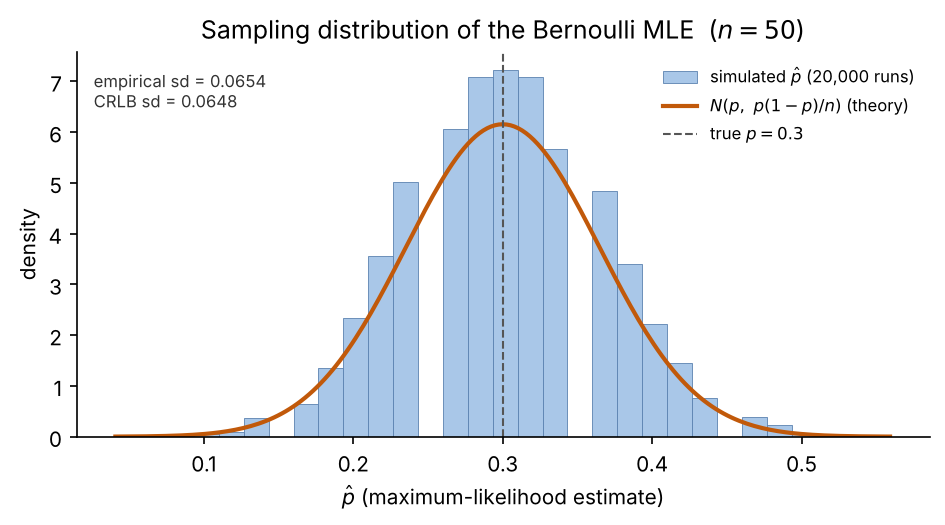
\includegraphics[width=0.82\textwidth]{figures/mle_sampling.png}
\end{figure}

\noindent The two numbers agree, and the picture says why: the histogram of
the estimates is already indistinguishable from the normal curve the
theorem predicts, and its spread sits on the Cram\'er--Rao floor. At $n=50$
the asymptotic result is not a distant promise --- it has already arrived.

% ======================================================================
\section{When the assumptions fail}
% ======================================================================

Every result above was stated ``under regularity.'' It is worth seeing
exactly what that phrase stands for, because it is not a formality: when it
breaks, the conclusions break with it. The conditions are that the support
of $f(\cdot\,;\theta)$ does not depend on $\theta$; that $\log f$ is twice
differentiable in $\theta$; that the derivative and the integral may be
exchanged; that $0<I_1(\theta)<\infty$; and that the true $\theta$ lies in
the interior of the parameter space.

\begin{example}[Where regularity fails: $\mathrm{Uniform}(0,\theta)$]
Here $f(x;\theta)=\tfrac1\theta\mathbf 1\{0\le x\le\theta\}$, and the support
\emph{does} depend on $\theta$, so the step that exchanges the derivative
and the integral is illegal. The MLE is $\hat\theta=\max_i x_i$, which is
biased, converges at rate $n$ rather than $\sqrt n$, and has an exponential
rather than a normal limiting distribution. The Cram\'er--Rao bound does not
apply at all. Regularity is doing real work in the theorems above.
\end{example}

There is also a broader way to read maximum likelihood that survives even
when the model is wrong. Writing $m(x;\theta)=\log f(x;\theta)$, the MLE
maximises the sample average $\frac1n\sum_i m(x_i;\theta)$. Estimators of
this ``optimise an average over the data'' form are called
\keyterm{M-estimators}, and the MLE is the special case $m=\log f$. By the
law of large numbers that average converges to $E_g[\log f(X;\theta)]$,
where $g$ is the \emph{true} data-generating density --- which need not be
any member of our model. Maximising it is the same as minimising
\[
  D_{\mathrm{KL}}(g \,\|\, f_\theta)
   = E_g\!\Big[\log \tfrac{g(X)}{f(X;\theta)}\Big],
\]
since the $E_g[\log g]$ piece does not involve $\theta$. So the MLE aims at
the parameter $\theta^\ast$ whose model is Kullback--Leibler closest to the
truth. If the model is correct, $\theta^\ast$ is the true parameter; if it
is wrong, the estimator still converges --- to the best approximation the
model can offer.

When the model is wrong the estimator is still asymptotically normal, but
its spread is no longer the simple $1/I_1$.

\begin{theorem}[Sandwich variance under misspecification]
When $g\notin\{f_\theta\}$,
\[
  \sqrt n(\hat\theta-\theta^\ast)\xrightarrow{d} N\!\big(0,\;A^{-1}BA^{-1}\big),
\]
with $A = -E_g[\partial_\theta^2 m]$ and
$B = \operatorname{Var}_g(\partial_\theta m)$. When the model is correct the
information identity gives $A=B=I_1$ and the two factors collapse to the
familiar $1/I_1$.
\end{theorem}

\begin{summarybox}
The MLE maximises $\ell(\theta)=\sum_i\log f(x_i;\theta)$. Its score has
mean zero, its precision is measured by the Fisher information, no unbiased
estimator can beat $1/I_n$ (Cram\'er--Rao), and in large samples it is
$N(\theta, 1/I_n)$ --- provided the regularity conditions hold and the model
is correct. Read as an M-estimator minimising a Kullback--Leibler
divergence, maximum likelihood is exactly what a classifier trained on
cross-entropy, or a density model trained on negative log-likelihood, is
doing. That is why this chapter sits under the loss-function chapter in
Part II.
\end{summarybox}

\end{document}
